% Copyright 2004 by Till Tantau <tantau@users.sourceforge.net>.
%
% In principle, this file can be redistributed and/or modified under
% the terms of the GNU Public License, version 2.
%
% However, this file is supposed to be a template to be modified
% for your own needs. For this reason, if you use this file as a
% template and not specifically distribute it as part of a another
% package/program, I grant the extra permission to freely copy and
% modify this file as you see fit and even to delete this copyright
% notice. 

\documentclass{beamer}

% There are many different themes available for Beamer. A comprehensive
% list with examples is given here:
% http://deic.uab.es/~iblanes/beamer_gallery/index_by_theme.html
% You can uncomment the themes below if you would like to use a different
% one:
%\usetheme{AnnArbor}
%\usetheme{Antibes}
%\usetheme{Bergen}
%\usetheme{Berkeley}
%\usetheme{Berlin}
%\usetheme{Boadilla}
%\usetheme{boxes}
%\usetheme{CambridgeUS}
%\usetheme{Copenhagen}
%\usetheme{Darmstadt}
%\usetheme{default}
%\usetheme{Frankfurt}
%\usetheme{Goettingen}
%\usetheme{Hannover}
%\usetheme{Ilmenau}
%\usetheme{JuanLesPins}
%\usetheme{Luebeck}
%\usetheme{Madrid}
%\usetheme{Malmoe}
%\usetheme{Marburg}
%\usetheme{Montpellier}
%\usetheme{PaloAlto}
%\usetheme{Pittsburgh}
%\usetheme{Rochester}
%\usetheme{Singapore}
%\usetheme{Szeged}
%\usetheme{Warsaw}

\usepackage{amsmath}
\usepackage{textpos}
\usepackage{ulem}
\usepackage{enumitem}

\definecolor{BYUblue}{RGB}{0,31,69}
\definecolor{BYUgold}{RGB}{195,163,106}
\usecolortheme[RGB={0,31,69}]{structure} % BYU Blue

\definecolor{metric-PR}{RGB}{200,127,0}
\definecolor{metric-NE}{RGB}{51,51,255}
\definecolor{metric-OFI}{RGB}{204,0,0}
\definecolor{metric-IRO}{RGB}{0,102,51}

\usetheme{Frankfurt}
\setbeamercolor*{section in head/foot}{bg=BYUblue,fg=gray!25}
\setbeamercolor*{frametitle}{bg=BYUblue!50,fg=white!25}
\setbeamercovered{transparent}
\mode<all>

\DeclareMathOperator*{\argmax}{arg\,max}

\title{MORRF$^{*}$: Sampling-based multi-objective path planning}

%\subtitle{Optional Subtitle}

\author{Daqing Yi 
%\and Michael A. Goodrich \and Kevin D. Seppi
}


\institute
{
  Department of Computer Science\\
  Brigham Young University
}

\date[]{} 

\addtobeamertemplate{frametitle}{}{%
\begin{textblock*}{100mm}(0.9\textwidth,-1.2cm)

\includegraphics[width=1.1cm]{figure/BYU_logo.png}
\end{textblock*}}

\begin{document}

\begin{frame}
  \titlepage
\end{frame}

\begin{frame}{Outline}{Structure}
  \tableofcontents
  % You might wish to add the option [pausesections]
\end{frame}

% Section and subsections will appear in the presentation overview
% and table of contents.

\section{Introduction}

\begin{frame}{Modeling human intent}{Path Planning}
THe problem in modeling human intent
\begin{itemize}
\item incomparability in objectives
\item conflict in objectives
\item hardness in weighing the objectives
\item vagueness in importance selection
\end{itemize}
\begin{figure}
\centering
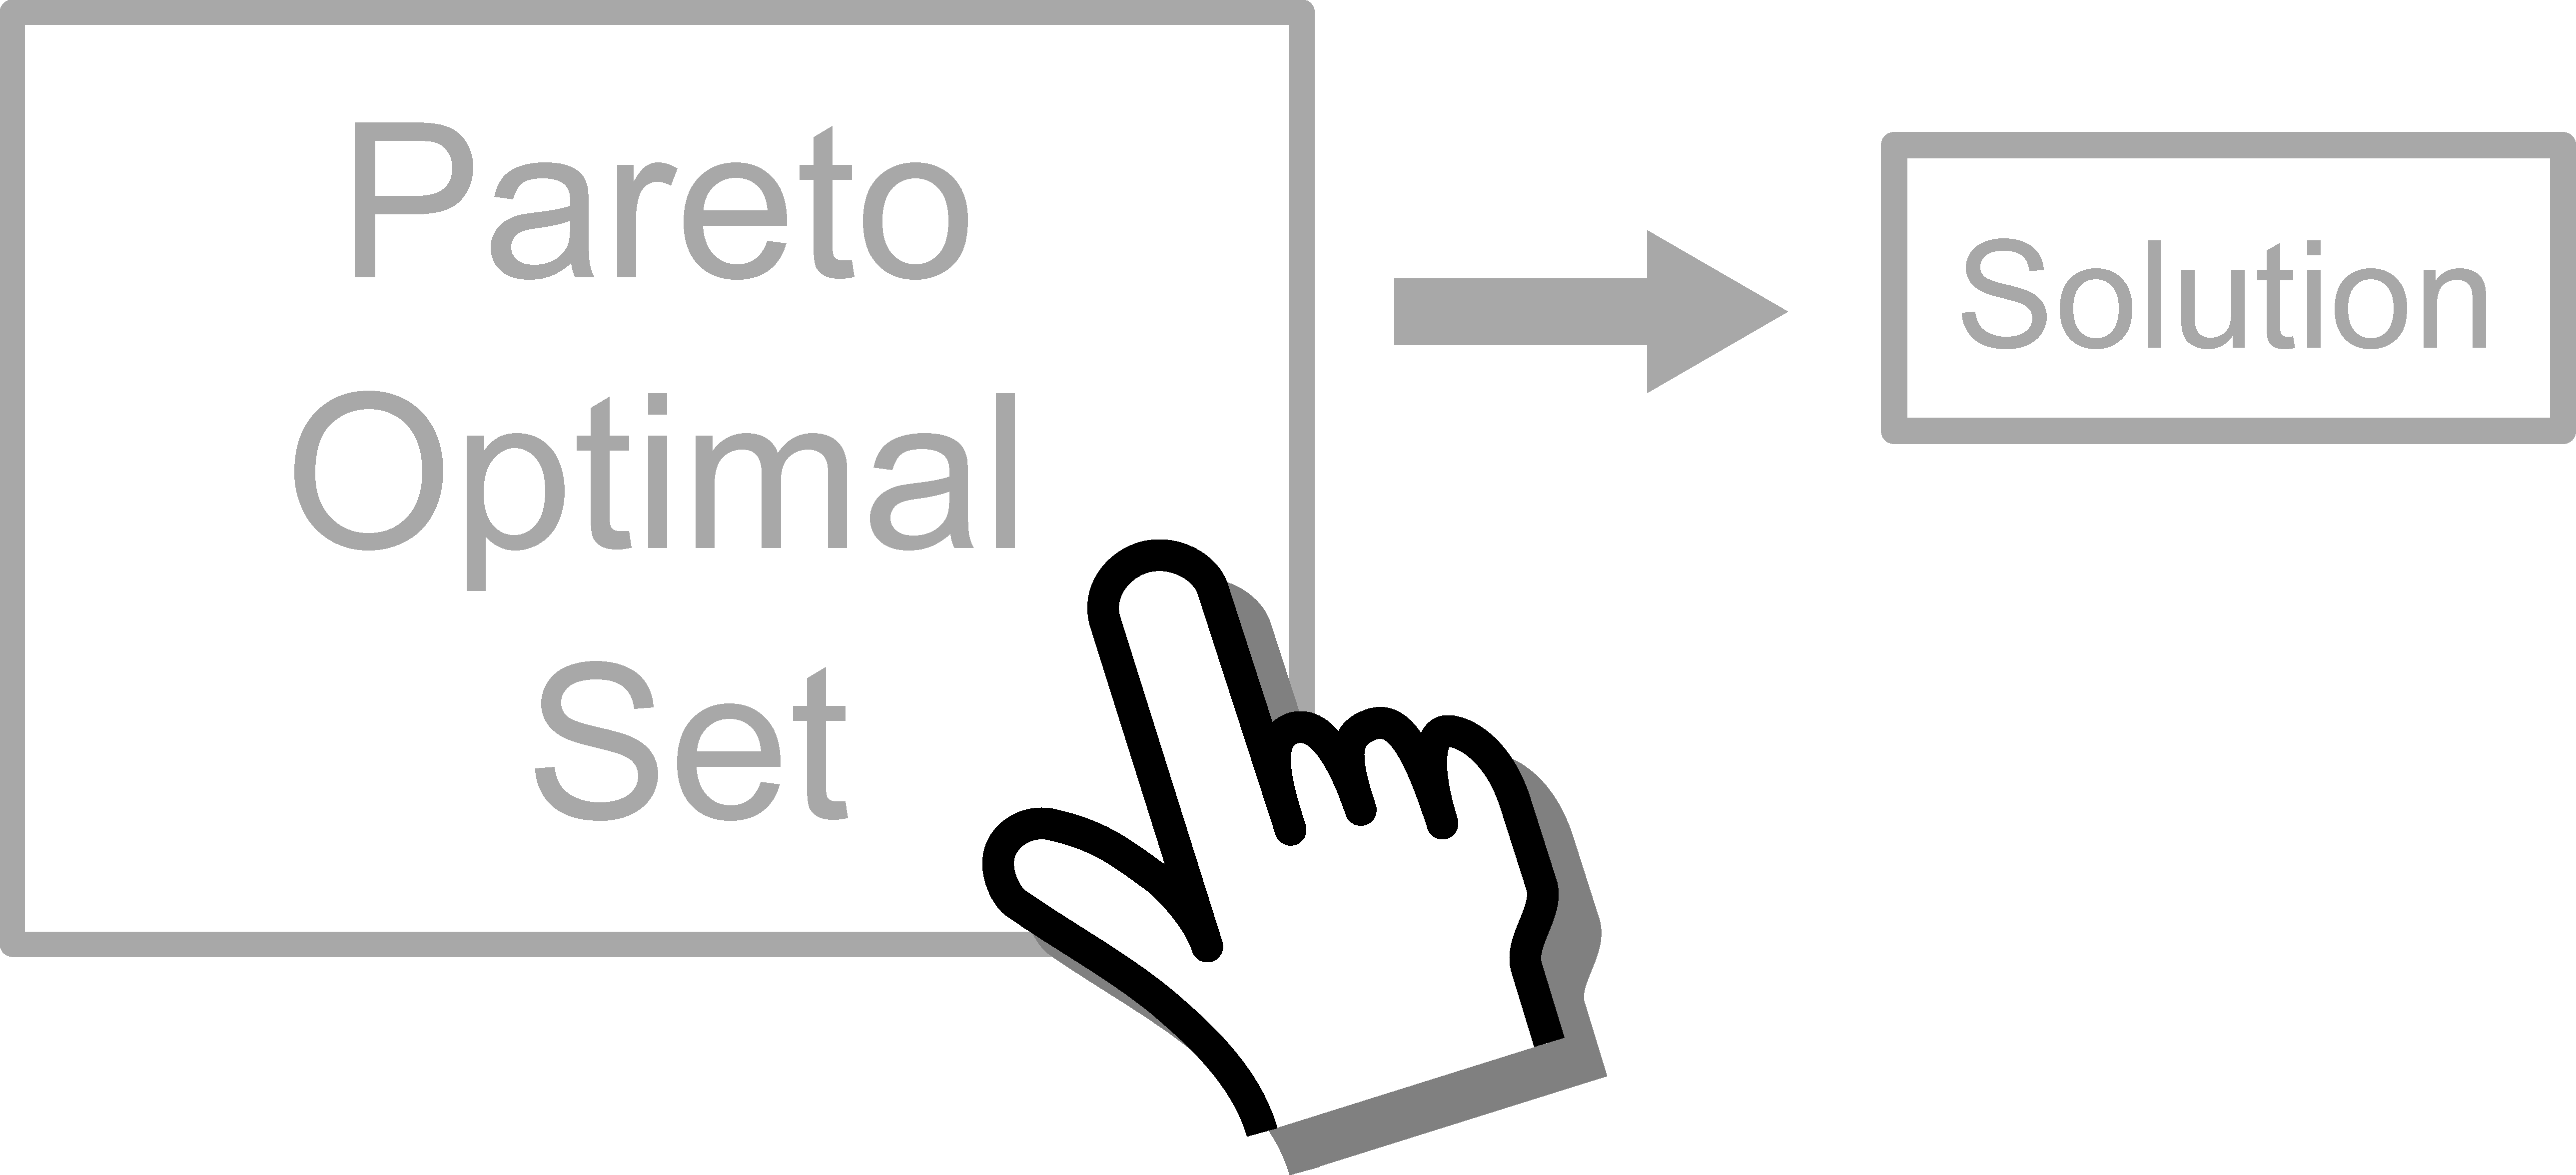
\includegraphics[width=0.6\linewidth]{figure/human_interactive_moo}
%\caption{}
\label{fig:human_interactive_moo}
\end{figure}
\end{frame}

\begin{frame}{Pareto Optimal}{}
\end{frame}

\section{Related work}

\begin{frame}{Graph based approach}{Related work}
Multi-objective A$ ^{*}$
\end{frame}

\begin{frame}{Point-equivalence based approach}{Related work}
\end{frame}



\section{Algorithm}

\subsection{probelm}

\begin{frame}{Multi-objective path planning}{Problem}
	
\begin{itemize}
\item a bounded, connected open set $ X \subset \mathbb{R}^{d} $
\item an obstacle space $ X_{obs} $
\item an initial state $ x_{init} $
\item a goal region $ X_{goal} $. 
\item $K$ objectives  $ \bm{c}(\cdot) = [ c_{1} (\cdot), \ldots , c_{K}(\cdot) ]^{T}$ 
\item the path  $\sigma : [0,s] \rightarrow X$. 
\end{itemize}

\textbf{problem} \\
find $ M $ Pareto optimal paths $ \sigma^{*} \in \Sigma^{*}$ 
\begin{itemize}
\item $\forall \tau\in[0,s], \sigma^*(\tau) \in X_{\it free}$;
\item $ \sigma^{*} (0) = x_{init} $ and $ \sigma^{*} (s) \in X_{goal}  $;
\item $ \nexists \sigma, \sigma \prec \sigma^{*} $     
\end{itemize}                        
	
\end{frame}

\subsection{algorithm}

\begin{frame}{Structure}{MORRF$^{*}$}
Multi-Objective Rapidly exploring Random Forest$^{*}$
\begin{itemize}
	\item \textbf{reference tree}
	\begin{itemize}
	\item One single objective
	\item Supporting the Utopia reference vector
	\end{itemize}	
	\item \textbf{subproblem tree}
	\begin{itemize}
	\item An assigned weight vector 
	\item Solving a sub-problem
	\end{itemize}
\end{itemize}
\end{frame}

\begin{frame}{Process}{MORRF$^{*}$}
\begin{figure}
	\centering
	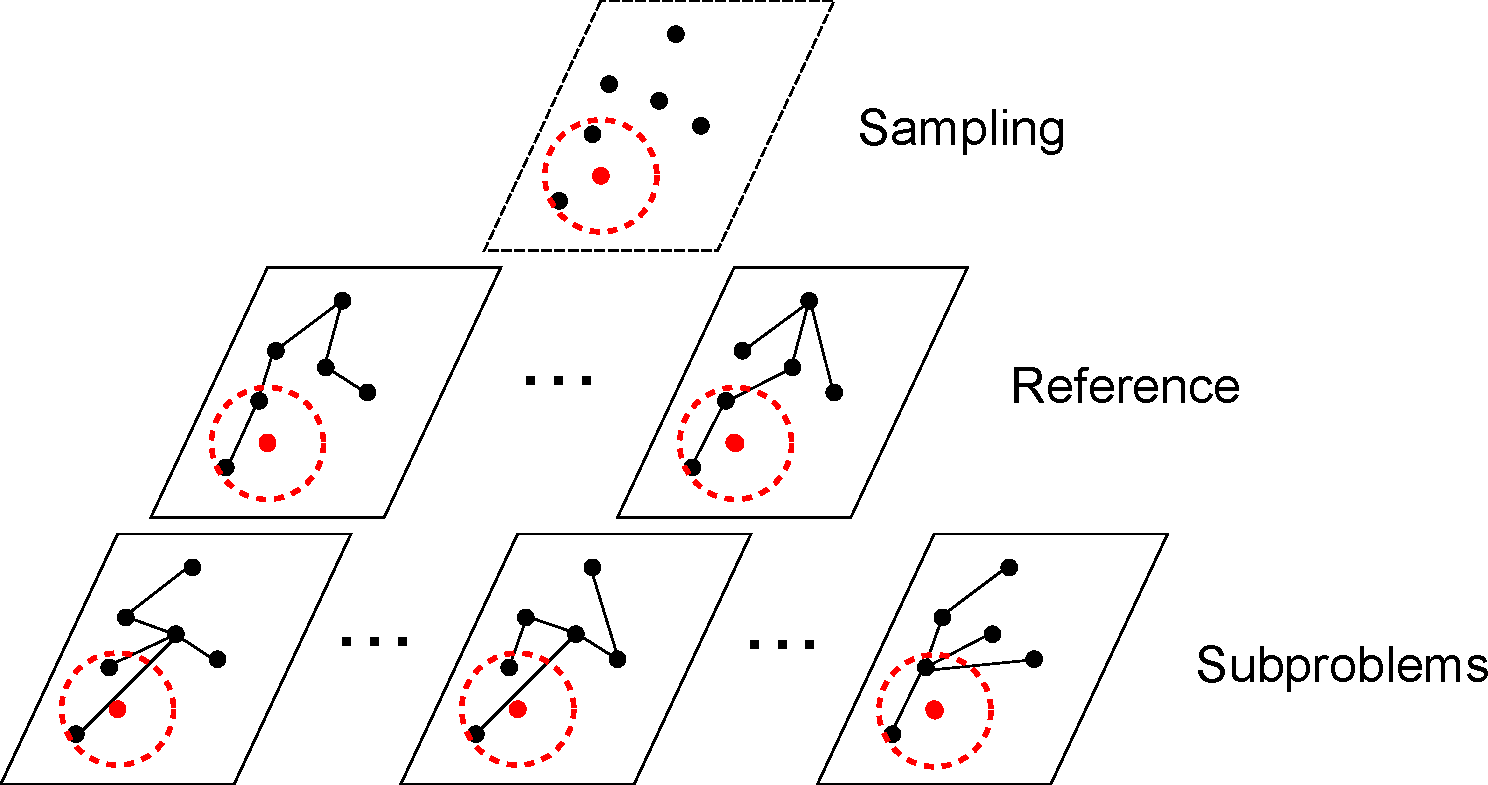
\includegraphics[width=.8\linewidth]{figure/MORRTstar.pdf}
	%\caption{}
	\label{fig:morrt:process}
\end{figure}
\end{frame}

\begin{frame}{Process}{MORRF$^{*}$}
	\begin{algorithmic}[1]
		\For{ \textbf{each} $ V_{r} \in \mathbf{V}_{r} $ } 
		\State $ V_{r} \leftarrow \{ x_{init} \} $; $ E_{r} \leftarrow \emptyset $; $ i \leftarrow 0 $
		\EndFor
		\For{ \textbf{each} $ V_{s} \in \mathbf{V}_{s} $ } 
		\State $ V_{s} \leftarrow \{ x_{init} \} $; $ E_{s} \leftarrow \emptyset $; $ i \leftarrow 0 $
		\EndFor
		\While{ $ i < N $ }
		%\For{ \textbf{each} $ G_{r} \in \mathbf{G}_{r} $ } 
		%\State $ G_{r} \leftarrow (V_{r}, E_{r}) $
		%\EndFor
		%\For{ \textbf{each} $ G_{s} \in \mathbf{G}_{s} $ } 
		%\State $ G_{s} \leftarrow (V_{s}, E_{s}) $
		%\EndFor
		\State $ x_{rand} \leftarrow $ \Call{ Sample }{$ i $} ; $ i \leftarrow i + 1 $
		%\State $ V' \leftarrow V $; $ E' \leftarrow E $
		\State $G$ is any graph from ${\mathbf G}_r\cup {\mathbf G}_s$.
		\State $ x_{nearest} \leftarrow $ \Call{Nearest}{$ G, x_{rand} $}
		\State $ x_{new} \leftarrow $ \Call{Steer}{$ x_{nearest}, x_{rand},\eta $}
		\If{ \Call{ObstacleFree}{$ x_{nearest}, x_{new} $} }
		\For{ \textbf{each} $ G_{r} \in \mathbf{G}_{r} $ } 
		%\State $ (V_{r}, E_{r}) \leftarrow $ \Call{ Extend$_{\it Ref}$ }{$ G_{r}, x_{new}, x_{\it nearest}, r$}
		\State $ G_{r} \leftarrow $ \Call{ Extend$_{\it Ref}$ }{$ G_{r}, x_{new}, x_{\it nearest}, r$}
		\EndFor
		\For{ \textbf{each} $ G_{s} \in \mathbf{G}_{s} $ } 
		%\State $ (V_{s}, E_{s}) \leftarrow $ \Call{ Extend$_{\it Sub}$ }{$ G_{s}, x_{new}, x_{\it nearest},s $}
		\State $ G_{s} \leftarrow $ \Call{ Extend$_{\it Sub}$ }{$ G_{s}, x_{new}, x_{\it nearest},s $}
		\EndFor
		\EndIf
		\EndWhile
	\end{algorithmic}
\end{frame}

\subsection{analysis}

\begin{frame}{Analysis}{MORRF$^{*}$}
\begin{columns}
	\column{0.5\textwidth}
	\begin{figure}
		\centering
		
\includegraphics[width=\linewidth]{figure/cascade}
		%\caption{}
		\label{fig:morrt:cascade}
	\end{figure}
	\column{0.4\textwidth}
	\begin{figure}
		\centering
		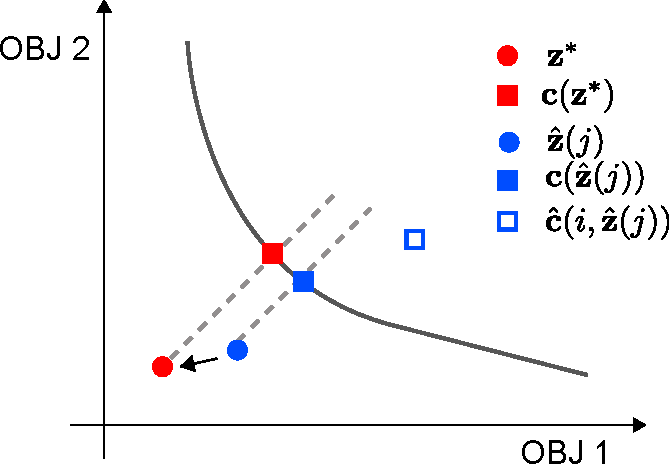
\includegraphics[width=\linewidth]{figure/conv}
		%\caption{}
		\label{fig:morrt:conv}
	\end{figure}
\end{columns}
\end{frame}

\begin{frame}{Analysis}{MORRF$^{*}$}

\begin{thm}
The solutions generated by MORRF$^{*}$ converges to a subset of the Pareto optimal set
almost surely.
\end{thm}

\end{frame}






\section{Conclusion}
\label{sec:conclusion}

In this paper, we have decomposed the PSO algorithm into a cascade model, which consists of input update and position update components.
We introduce the input-to-state stability analysis to the position update component.
For an input-to-state stable position update component, if the input to this component is bounded, the state is bounded; also if the input to the component converges, the state converges.
The convergence of the PSO is determined by the output of the input update component, which are the personal best and global best.
If they are in stagnation, the particle converges.

The analysis of a cascade structure used here can be applied to a wide range of the PSO variants.
In cases that use the same position update component but different input update components, the convergence and the boundary of the particles are determined by
whether the input update component generates converging or bounded personal best and global best.
For variants that use a different position update component, the ISS properties would need to be verified.



\end{document}


